% hello.tex - Our first LaTeX example!

\documentclass{article}
\usepackage{graphicx}

\begin{document}

Santiago Cuesta 201073571-0\\
Pablo Castro 201073521-4\\

En un comienzo internet fue creado con un prop�sito militar, luego se le dio un uso cient�fico y finalmente se convirti� en la red de redes que conocemos hoy en d�a. Internet es considerada una ?red de redes? que permite la interconexi�n de distintos dispositivos mediante el protocolo TCP/IP.\\\\
Existen muchos proveedores de internet, los llamados ISP(Internet Service Provider), que son empresas que brindan  conexi�n a internet a sus clientes utilizando distintos tipos de enlaces, cada uno con caracter�sticas espec�ficas. A grandes rasgos los podemos separar en 3 grupos:\\\\
1) ISP nivel 1: son proveedores de internet que proporcionan cobertura a nivel internacional. Estos se conectan directamente con otros ISP nivel 1 y est�n conectados a un gran n�mero de ISP nivel 2. Tienen una velocidad de enlace superior a 622 Mbps (rango entre 2.5 y 10 Gbps). Algunos de estos son AOL, AT\&T, Global Crossing.\\\\
2) ISP nivel 2: son proveedores de internet que proporcionan cobertura a nivel regional o nacional. Estos se conectan a ISP nivel 1 y a otros ISP nivel 2 (no es necesario pasar por un ISP nivel 1 para conectarse con otro ISP nivel 2). Algunos de estos (que operan en chile) son VTR, Movistar y Claro.\\\\
3) ISP nivel inferior: son las redes de acceso.\\\\
La conexi�n entre chile y el resto del mundo se hace por medio de enlaces de fibra �ptica. Estos enlaces est�n ubicados en Arica y Valpara�so. Estos son:\\\\
a)	South America-1 (Sam-1): Arica y Valpara�so.\\
b)	Pan American (PAN AM):  Arica.\\
c)	South American Crossing (SAC)/Latin American Nautilus (LAN): Valpara�so.\\\\
Finalmente, los paquetes enviados de un host a otro deben pasar por una serie de routers, dependiendo de la ubicaci�n existente entre ambos host y de que tan saturada se encuentre una ruta.\\
Con lo explicado anteriormente y utilizando la aplicaci�n OpenVisualTraceRoute, veamos que sucede al ingresar diferentes direcciones.\\\\\\\\\\\\\\\\

Direcciones:\\\\ 
\begin{figure}[ht!]
\centering
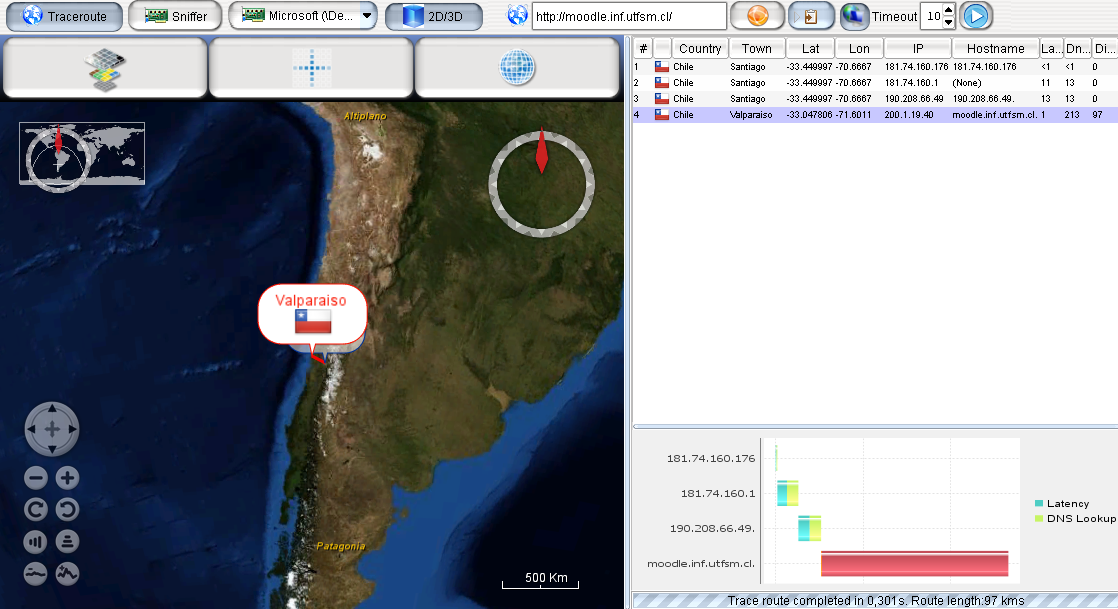
\includegraphics[width=100mm]{moodle_inf_utfsm_cl.png}
\caption{http://moodle.inf.utfsm.cl/ }
\label{overflow}
\end{figure}\\
Como se puede apreciar, el servidor en el que est� alojada esta direcci�n se encuentra en Valpara�so, por lo tanto una ruta �ptima no considerar�a necesario pasar por ISP de nivel 1, ya que ambos host se encuentran en el mismo pa�s. \\
\begin{figure}[ht!]
\centering
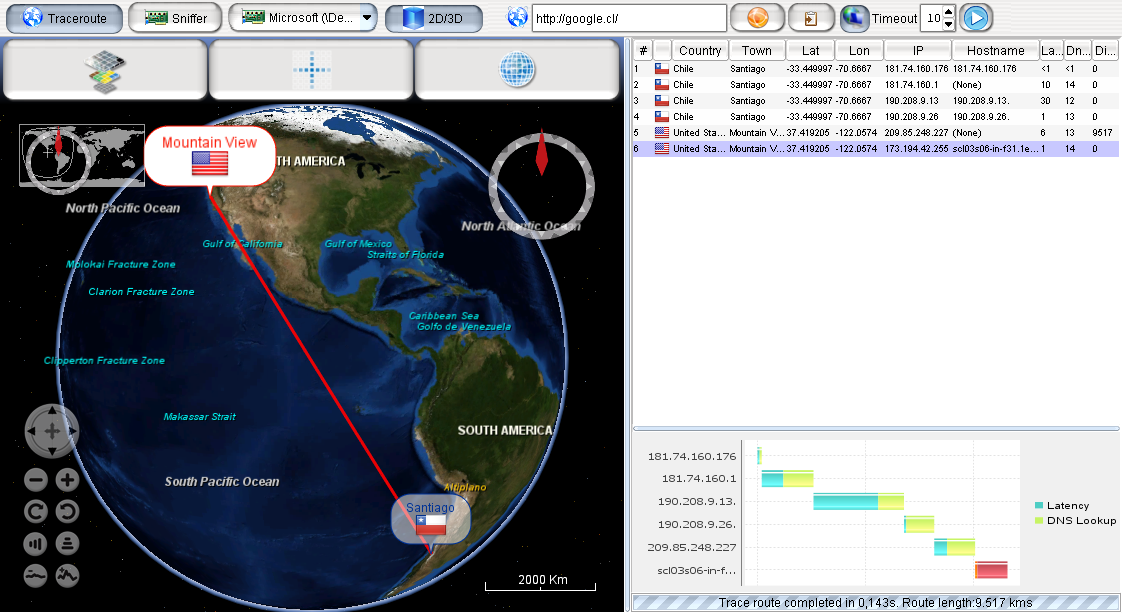
\includegraphics[width=100mm]{google_cl.png}
\caption{http://google.cl/ }
\label{overflow}
\end{figure}\\
Ac� podemos apreciar que el servidor en el que est� alojada esta direcci�n, a diferencia del caso anterior, no se encuentra en Chile, por lo tanto es necesaria una conexi�n internacional con un ISP nivel 1. Tambi�n podemos apreciar que el servidor de google se encuentra en Mountain View, Estados Unidos.\\
\begin{figure}[ht!]
\centering
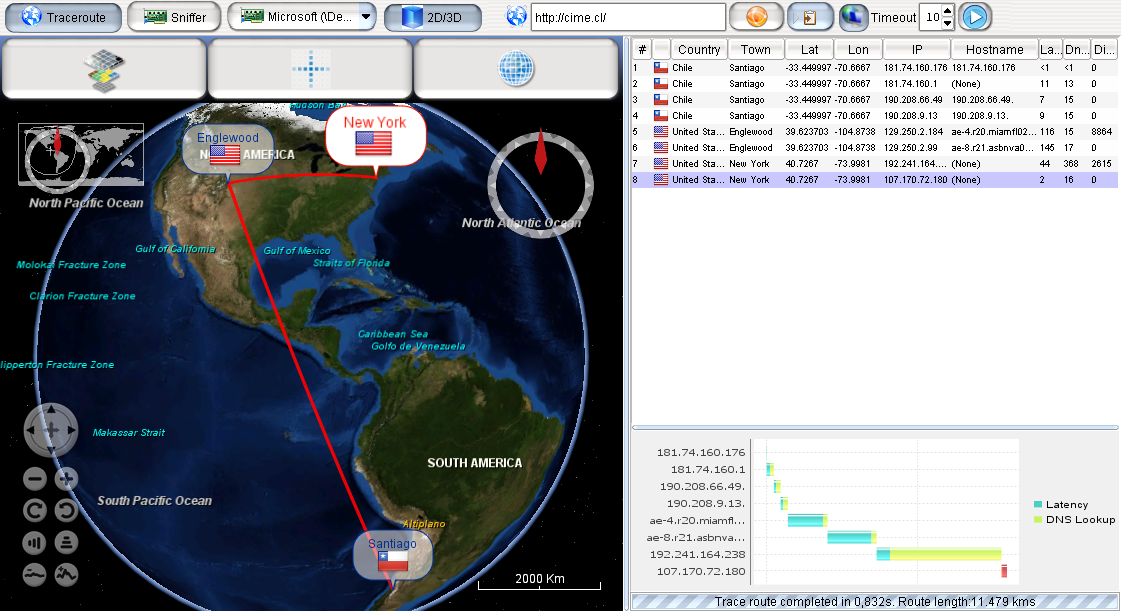
\includegraphics[width=100mm]{cime_cl.png}
\caption{http://cime.cl/ }
\label{overflow}
\end{figure}\\
En el caso de cime.cl notamos que el servidor se encuentra fuera del pa�s, por lo tanto, al igual que en el caso de google en necesaria la conexi�n con un ISP nivel 1. Tambi�n podemos ver que el servidor se encuentra en New York, y para llegar a �l no existe una conexi�n directa entre Santiago y este, por lo tanto debe pasar primero por Eaglewood.\\
\begin{figure}[ht!]
\centering
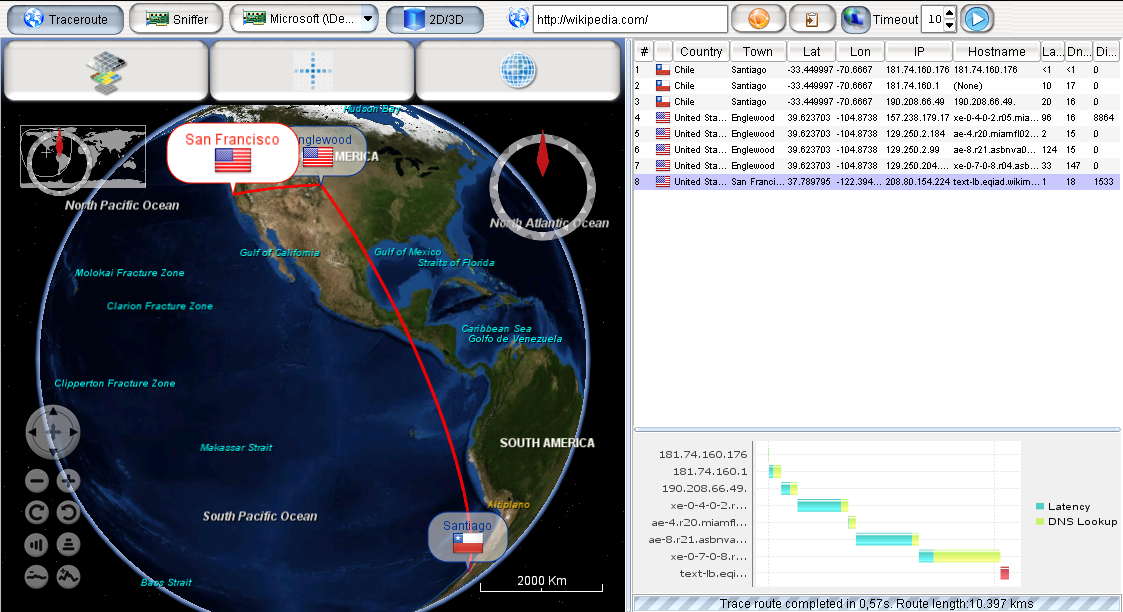
\includegraphics[width=100mm]{wikipedia_com.png}
\caption{http://wikipedia.com/ }
\label{overflow}
\end{figure}\\
Para el caso de Wikipedia ocurre algo similar a cime.cl, ya que el servidor se encuentra en Estados Unidos, pero no existe conexi�n directa entre San Francisco y Santiago. Nuevamente es necesario pasar por Eaglewood para acceder al comunicarse con el host destino.\\
\begin{figure}[ht!]
\centering
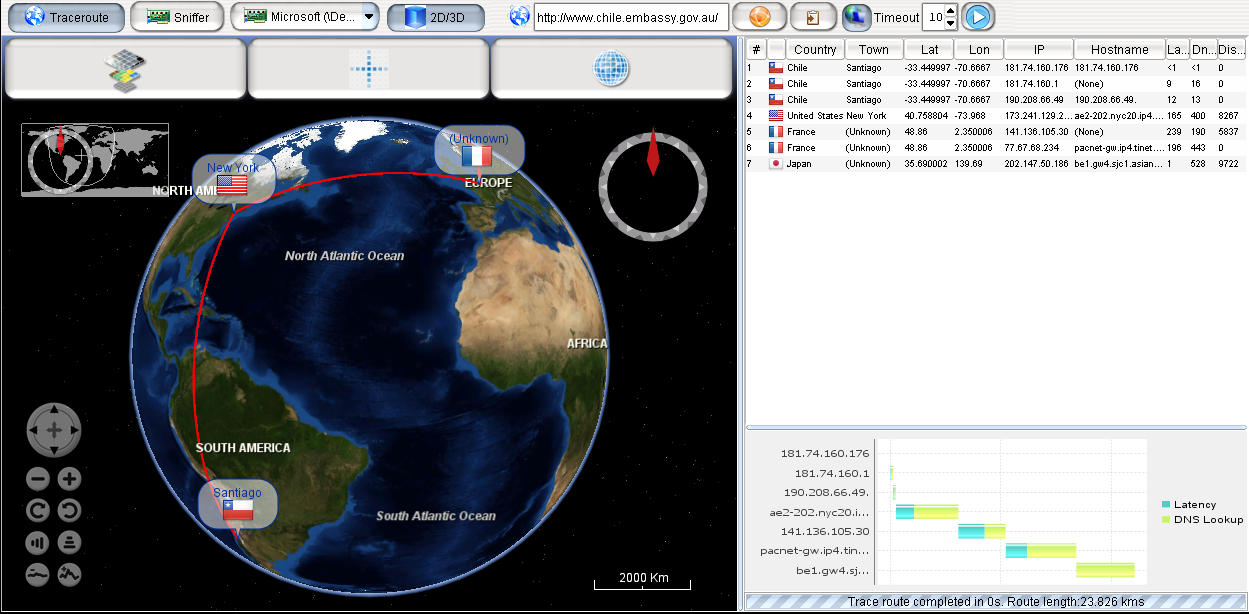
\includegraphics[width=100mm]{www_chile_embassy_gov_1.png}
\caption{http://www.chile.embassy.gov.au/ }
\label{overflow}
\end{figure}\\
\begin{figure}[ht!]
\centering
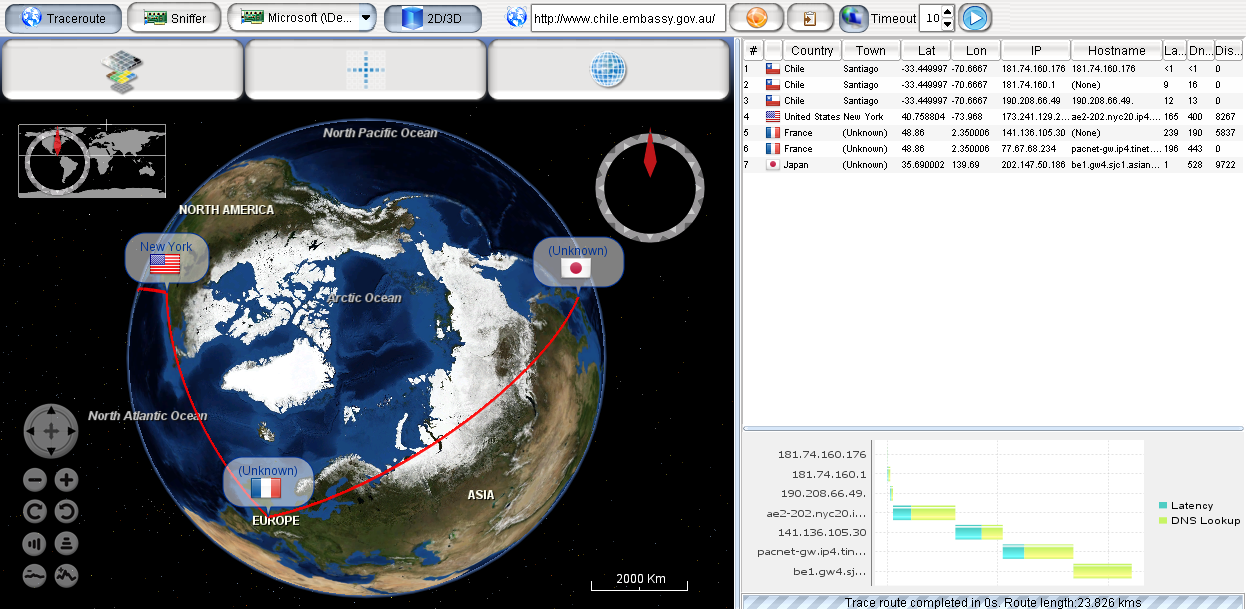
\includegraphics[width=100mm]{www_chile_embassy_gov_2.png}
\caption{http://www.chile.embassy.gov.au/ }
\label{overflow}
\end{figure}\\
Finalmente para el caso de esta direcci�n notamos que pasa por diferentes pa�ses hasta llegar a su destino. Esto es as� ya que no existe una conexi�n directa entre ambos host. La ruta �ptima encontrada por OpenVisualTraceRoute  considera el paso desde Chile a Estados Unidos, luego a Francia, para finalmente llegar a Jap�n. A diferencia de las direcciones anteriores, aqu� se realiza una comunicaci�n intercontinental por medio de un cable submarino que atraviesa el oceano.\\

\end{document}
		